\subsection{Generic ARQ implementation}\label{sc:overall}

The ARQ stop-and-wait method has been implemented on all nodes in the system. Figure \ref{fig:tohopornotarqsequence} is a sequence diagram of the  protocol implementation and shows how data requests are initiated by the base station and forwarded either directly to the runner (left side) or via a relay station (right side). Adding to this is the parity bit calculations to verify the integrity of received frames. This is conduced when a frame is received in either base station or one of the other nodes.

\begin{figure}[H]
	\centering
	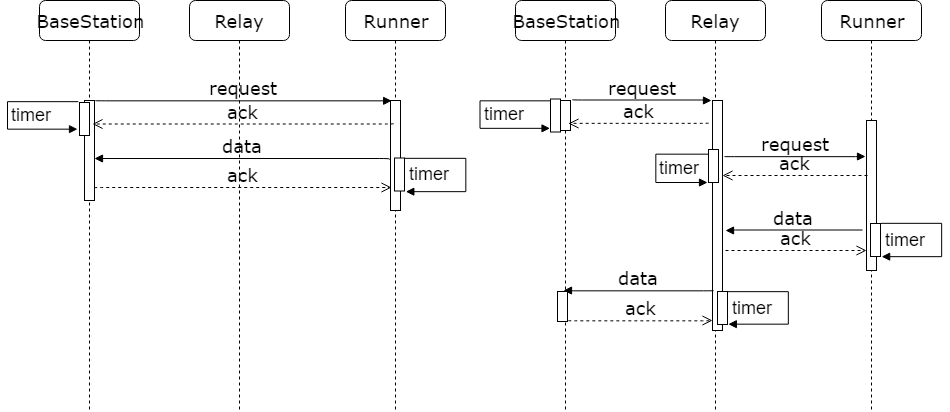
\includegraphics[width=1\linewidth]{implementation/overall/toHopOrNotArqSequence}
	\caption{The flow of data and acknowledgment messages between the nodes.}
	\label{fig:tohopornotarqsequence}
\end{figure}

\noindent The basics of the communications between the nodes are as follows: \\ \newline
1. The base station requests data at a certain time interval defined by a timer. When the timer runs out, it decides whether is should send the request directly or via one of the relays by using our protocol. To the request is attached a counter ($n = 0, 1, 2, 3$ -> $n$) and a sequence number (0 or 1) used by the receiver to verify the frame. When the radio is ready to transmit, it is forwarded to a specific node and the ARQ timer starts. It it now the responsibility of the receiving node to carry on the request. The receiver will send back a ACK frame to the base station if validation succeeded.\\ \newline
2. If the request reached the runner first, it will use the attached counter to calculate a new parity bit and compare this to the one in the request. If they match, it sends back an ACK followed by a data message containing the current heart rate of the athlete. A counter and a sequence number is attached to this as well.\\ \newline
3. The base station receives the data message, checks the parity bit, and saves it. It has now successfully obtained the heart rate.\\ \newline
4. If the base station decide to relay the request, the same procedure applies for the relay nodes. It is now the job of the relay to acknowledge the request, communicate with the runner using ARQ, obtain the data and send it back to the base station.\\ \newline
\noindent With ARQ and parity bit checking we archive a simple but reliable data-link connection between nodes and a way to discard damaged frames. One particular area of concern was the configuration of the timers, as they have to be consistent throughout the network. Obviously when relaying, the base station must take into account the turnaround time and possible retransmissions of the relay and the runner node before sending a new one. The base station timer ($Ba_t$) must be larger than the relay's ($Re_t$) and the runner's ($Ru_t$) combined, so $Ba_t$ > $Re_t$ + $Ru_t$ for the protocol to work correctly.